\usepackage{amsmath}
\usepackage{amsfonts}
\usepackage{amssymb}
\usepackage{graphicx}
\usepackage{blindtext}
\usepackage{textcomp}
\usepackage{pgfplots}

\pgfplotsset{width=10cm,compat=1.9}


%Header styles
\usepackage{fancyhdr}
\setlength{\headheight}{15pt}
\pagestyle{fancy}
\renewcommand{\sectionmark}[1]{\markright{#1}{}}
\fancyhf{}
\fancypagestyle{plain}{ %
\fancyhf{} % remove everything
\renewcommand{\headrulewidth}{0pt} % remove lines as well
\renewcommand{\footrulewidth}{0pt}}

%makes available the commands \proof, \qedsymbol and \theoremstyle
\usepackage{amsthm}

%Ruler
\newcommand{\HRule}{\rule{\linewidth}{0.5mm}}

%Commands for naturals, integers, topology, hull, Ball, Disc, Dimension, boundary and a few more
\newcommand{\E}{{\mathcal{E}}}
\newcommand{\F}{{\mathcal{F}}}
\newcommand{\T}{{\mathcal{T}}}
\newcommand{\Bs}{{\mathcal{B}}}
\newcommand{\R}{{\mathbb{R}}}
\newcommand{\Q}{{\mathbb{Q}}}
\newcommand{\Z}{{\mathbb{Z}}}
\newcommand{\Nt}{{\mathbb{N}}}
\newcommand{\B}{{\mathbf{B}}}
\renewcommand{\S}{{\mathbf{S}}}
\newcommand{\K}{{\mathfrak{C}}}
\newcommand{\N}{{\mathfrak{N}}}
\newcommand{\I}{{\mathbf{I}}}
\newcommand{\dime}{{\rm dim}\,}
\newcommand{\est}{{\rm Est}\,}
\newcommand{\inte}{{\rm int}\,}
\newcommand{\conv}{{\rm conv}\,}
\renewcommand{\max}{{\rm sup\,}}
\newcommand{\diam}{{\rm di\acute{a}m\,}}
\newcommand{\leyenda}[1]{\caption{{\small \textsf{#1}}}}
\renewcommand{\inf}{{\rm \acute{i}nf}\,}

\usepackage[margin=1in]{geometry} 
\usepackage{amsmath}
\usepackage{tcolorbox}
\usepackage{indentfirst}
\usepackage{amssymb}
\usepackage{amsthm}
\usepackage{lastpage}
\usepackage{fancyhdr}
\usepackage{enumitem}
\usepackage{accents}
\usepackage{blindtext}
\usepackage{booktabs}
\usepackage{enumitem}
\usepackage{mathtools}
\pagestyle{fancy}
\setlength{\headheight}{40pt}
\usepackage[utf8]{inputenc}
\usepackage[russian]{babel}
\everymath{\displaystyle}
\usepackage{cancel}
\geometry{verbose,a4paper,tmargin=2cm,bmargin=2cm,lmargin=1cm,rmargin=1.5cm}

\usepackage{hyperref}
\hypersetup{
    colorlinks,
    citecolor=black,
    filecolor=black,
    linkcolor=blue,
    urlcolor=blue
}

\newenvironment{solution}
  {\renewcommand\qedsymbol{$\blacksquare$}
  \begin{proof}[Solution]}
  {\end{proof}}
\renewcommand\qedsymbol{$\blacksquare$}

\newtheorem{theorem}{Теорема}
\newtheorem{lemma}{Лемма}
\newtheorem{statement}{Утверждение}
\newtheorem{corollary}{Следствие}
\newtheorem{advice}{Предложение}

\theoremstyle{definition}
\newtheorem{example}{Пример}

\theoremstyle{definition}
\newtheorem{definition}{Определение}

\theoremstyle{remark}
\newtheorem{remark}{Замечание}

\theoremstyle{definition}
\newtheorem*{reminder}{Напоминание}

\newcommand{\ubar}[1]{\underaccent{\bar}{#1}}

\DeclarePairedDelimiter\abs{\lvert}{\rvert}%

\makeatletter
\let\oldabs\abs
\def\abs{\@ifstar{\oldabs}{\oldabs*}}



\begin{document}

\lhead{Иванов Семен} 
\rhead{БПМИ-183} 
\cfoot{\thepage\ of \pageref{LastPage}}

\section{Листок 3. Задача 12}

\begin{itemize}
\item Пусть $R_X = \text{cov}\left(X, X\right)$.
% \item Ортонормируем $X_1, X_2$. Применим метод Грама-Шмидта к подпространству $\left(X_1, X_2\right)$ со скалярным произведением $\left(X, Y\right) = E XY$:
% \[
%     b_1 = X_1
% \]
% \[
%     b_2 = X_2 - pr_{b_1} X_1 = X_2 - \frac{\left(X_2, X_1\right)}{\left(X_1, X_1\right)}X_1 = X_2 - \frac{\text{cov}\left(X_2, X_1\right)}{\text{cov}\left(X_1, X_1\right)} X_1 = -\frac 1 2 X_1 + X_2
% \]
% Теперь отнормируем вектора:
% \[
%     Y_1 = \frac{b_1}{\sqrt{\left(b_1, b_1\right)} }= \frac{b_1}{\sqrt{3}} = \frac{X_1}{\sqrt{3}}
% \]
% \[
%     Y_2 = \frac{b_2}{\sqrt{\left(b_2, b_2\right)}} = \frac{b_2}{\sqrt{2 + \frac 1 4 \cdot 3   - 2 \cdot \frac 1 2 \cdot 3}} = \frac{2b_2}{\sqrt{7}} = -\frac{X_1}{\sqrt{7}} + \frac{2X_2}{\sqrt{7}}
% \]

% \item Теперь имеем:
% \[
%     \begin{pmatrix}
%     \frac {1} {\sqrt {3}} & 0 \\
%     -\frac {1} {\sqrt{7}} & \frac{2}{\sqrt{7}}
%     \end{pmatrix}
%     \begin{pmatrix}
%     X_1 \\
%     X_2
%     \end{pmatrix} = 
%     \begin{pmatrix}
%     e_1 \\
%     e_2
%     \end{pmatrix}
% \]
% \[
%     \begin{pmatrix}
%     X_1 \\
%     X_2
%     \end{pmatrix} = 
%     \begin{pmatrix}
%     \sqrt 3 & 0 \\
%     \frac{\sqrt{3}}{2} & \frac{\sqrt{7}}{2}
%     \end{pmatrix}
%     \begin{pmatrix}
%     e_1 \\
%     e_2
%     \end{pmatrix},
% \]
%  где $e_1, e_2 \sim N\left(0, 1\right) \ - $ независимые случайные величины.

 \item Так как 
 \[
    A 
    \begin{pmatrix}
        X_1 \\ X_2
    \end{pmatrix} = 
    \begin{pmatrix}
        1 & a \\ 0 & 1
    \end{pmatrix} \begin{pmatrix}
        X_1 \\ X_2
    \end{pmatrix} = \begin{pmatrix}
        X_1 + aX_2 \\ X_2
    \end{pmatrix},
 \]
 то $\left(X_1 + aX_2, X_2\right) \sim N\left(0, AR_X A ^ T\right)$.
 \[
    A R_X A ^ T = \begin{pmatrix}
    3 + 2a + 2a ^ 2 & 1 + 2a \\ 
    1 + 2a & 2
    \end{pmatrix}
 \]
 \item На лекции была теорема: если вектор $\left(X_1 + aX_2, X_2\right)$ имеет нормальное распределение и $\text{cov}\left(X_1 + aX_2, X_2\right) = 1 + 2a = 0$, то случайные величины $X_1 + aX_2$ и $X_2$ независимы. Получаем, что $a = -\frac 1 2 $.
\end{itemize}

\section{Листок 3. Задача 8b*}

\begin{itemize}
\item Из прошлого номера мы выразили случайный вектор $\left(\xi, \eta\right)$ через независимые стандартные случайные величины $e_1$ и $e_2$ ($a, c > 0$ по понятным причинам $ -$ потому что в прошлом номере там корни):
\[
    \begin{pmatrix}
    \xi \\ \eta
    \end{pmatrix} = 
    \begin{pmatrix}
    a & 0 \\ b & c
    \end{pmatrix} 
    \begin{pmatrix}
    e_1 \\ e_2
    \end{pmatrix}
\]
\item Теперь найдем
\[
    P\left(\xi \geq 0, \eta \geq 0\right) = P\left(ae_1 \geq 0, b e_1 + c e_2 \geq 0\right) = P\left(e_1 \geq 0, e_2 \geq -\frac{be_1}{c}\right) = 
\]
\[
    = \int_{0}^{+\infty} \int_{-\frac{bx}{c}}^{+\infty} \rho_{e_1, e_2}\left(x, y\right) dy dx = 
    \frac 1 {2\pi} \int_{0}^{+\infty} \int_{-\frac{bx}{c}}^{+\infty} e ^ {-\frac{x ^ 2 + y ^ 2}{2}} dy dx = 
\]
Сделаем полярную замену
\[
    =  \frac 1 {2\pi} \int_{0}^{+\infty} \int_{- \arctg\left(\frac b c\right)}^{\frac \pi 2} e ^ {-\frac{r ^ 2}{2}} r d\varphi dr
    = \frac{\frac{\pi}{2} + \arctg\left(\frac b c\right)}{4\pi} \int_{0}^{+\infty} e ^ {-\frac{r ^ 2}{2}} d \left(r ^  2\right) = \frac{\frac{\pi}{2} + \arctg\left(\frac b c\right)}{2\pi}
\]
\item Аналогично
\[
    P\left(\xi \leq 0, \eta \leq 0\right) = 
    \int_{-\infty}^{0} \int_{-\infty}^{-\frac{bx}{c}} \rho_{e_1, e_2}\left(x, y\right) dy dx = \frac 1 {2\pi} \int_{0}^{+\infty} \int_{\pi - \arctg\left(\frac b c\right)}^{\frac {3\pi} 2} e ^ {-\frac{r ^ 2}{2}} r d\varphi dr = \frac{\frac{\pi}{2} + \arctg\left(\frac b c\right)}{2\pi}
\]
\item 
\[
    P\left(\xi \leq 0, \eta \geq 0\right) = 
    \int_{-\infty}^{0} \int^{+\infty}_{-\frac{bx}{c}} \rho_{e_1, e_2}\left(x, y\right) dy dx = 
    \frac 1 {2\pi} \int_{0}^{+\infty} \int^{\pi - \arctg\left(\frac b c\right)}_{\frac {\pi} 2} e ^ {-\frac{r ^ 2}{2}} r d\varphi dr = \frac{\frac \pi 2 - \arctg\left(\frac b c\right)}{2\pi}

\]
\item 
\[
    P\left(\xi \geq 0, \eta \leq 0\right) = 
    \int^{+\infty}_{0} \int_{-\infty}^{-\frac{bx}{c}} \rho_{e_1, e_2}\left(x, y\right) dy dx = 
    \frac 1 {2\pi} \int_{0}^{+\infty} \int_{\pi - \arctg\left(\frac b c\right)}^{\frac {3\pi} 2} e ^ {-\frac{r ^ 2}{2}} r d\varphi dr = \frac{\frac \pi 2 - \arctg\left(\frac b c\right)}{2\pi}

\]
 
\end{itemize}


\section{Листок 4. Задача 4}
 Посчитатем распределение $\eta$, используя свойства условного матожидания:
\[
    P\left(\eta = s\right) = \mathbb{E}\text{Ind}_{\eta = s} = \mathbb{E}\left[\mathbb{E}\left(\text{Ind}_{\eta = s} | \xi\right)\right] = \sum_{k = 0}^{\infty} P\left(\xi = k\right) \mathbb{E}\left(\text{Ind}_{\eta = s} | \xi = k\right) = \sum_{k = s}^{\infty} P\left(\xi = k\right) \mathbb{E}\left(\text{Ind}_{\eta = s} | \xi = k\right) = 
\]
\[
    = \sum_{k = s}^{\infty} \frac{\lambda ^ k e ^ {-\lambda}}{k!} P\left(\text{Ind}_{\eta = s} = 1 | \xi = k\right) = \sum_{k = s}^{\infty} \frac{\lambda ^ k e ^ {-\lambda}}{k!} {{k}\choose{s}} p ^ s \left(1 - p\right) ^ {k - s} = p ^ s e ^ {-\lambda} \sum_{k = s}^{\infty} \frac{\lambda ^ k k! \left(1 - p\right) ^ {k - s}}{k! s! \left(k - s\right)!} = 
\]
\[
    = \frac{\lambda^ s p ^s e ^ {-\lambda}}{s!} \sum_{k = s}^{\infty} \frac{\lambda ^ {k - s}\left(1 - p\right) ^ {k - s}}{\left(k - s\right)!} = \frac{\lambda^ s p ^s e ^ {-\lambda}}{s!} \sum_{k = 0}^{\infty} \frac{\lambda ^ k \left(1 - p\right) ^ {k}}{k!} = \frac{\lambda^ s p ^s e ^ {-\lambda p}}{s!} \sum_{k = 0}^{\infty} \frac{\left(\lambda \left(1 - p\right)\right) ^ {k} e ^ {-\lambda\left(1 - p\right)}}{k!}
\]
Заметим, что
\[
    \sum_{k = 0}^{\infty} \frac{\left(\lambda \left(1 - p\right)\right) ^ {k} e ^ {-\lambda\left(1 - p\right)}}{k!} =1
\]
так как это сумма вероятностей $P\left(\zeta = k\right)$, где $\zeta \sim Poiss\left(\lambda\left(1 - p\right)\right)$. Таким образом, получаем 
\[
    P\left(\eta = s\right) = \frac{\left(\lambda p\right) ^s e ^ {-\lambda p}}{s!},
\]
то есть $\eta \sim Poiss\left(\lambda p\right)$
\qed

\section{Листок 4. Задача 9}

\begin{itemize}
\item Для совместного распределения просто заполним табличку $P\left(X = x, Y = y\right)$: \\
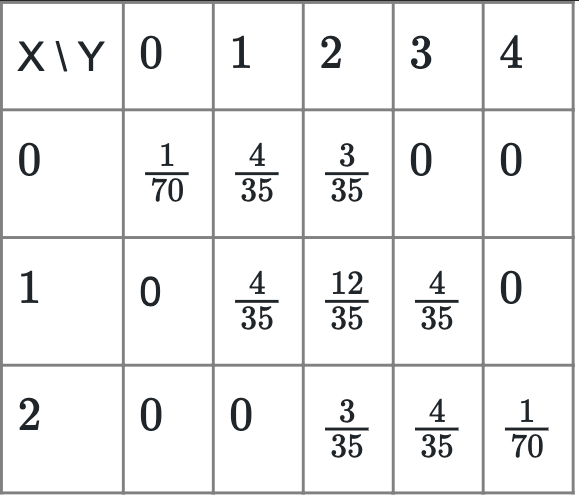
\includegraphics[width=193pt]{img1.png}
\item $P\left(Y = 3\right) = 0 + \frac{4}{35} + \frac{4}{35} = \frac{8}{35}$ (нашли из таблицы). Находим условное распредление:
\[
    P\left(X = 0 | Y = 3\right) = \frac{P\left(X = 0, Y = 3\right)}{P\left(Y = 3\right)} =0 
\]
\[
    P\left(X = 1 | Y = 3\right) = \frac{P\left(X = 1, Y = 3\right)}{P\left(Y = 3\right)} = \frac 1 2
\]
\[
    P\left(X = 2 | Y = 3\right) = \frac{P\left(X = 2, Y = 3\right)}{P\left(Y = 3\right)} = \frac 1 2
\]
\item Находим условные ожидания по определению:
\[
    \mathbb{E}\left(X | Y\right) = 
    \begin{cases}
    0, & Y = 0 \\
    \frac 1 2, & Y = 1 \\
    1, & Y = 2 \\
    \frac 3 2, & Y = 3 \\
    2, & Y = 4 
    \end{cases}
\]
\[
    \mathbb{E} \left(Y | X\right) = 
    \begin{cases}
    \frac 4 3, & X = 0 \\
    2 ,& X = 1\\
    \frac 8 3 ,& X = 2
    \end{cases}
\]
\end{itemize}

\section{Листок 3. Задача 8с(ромбик)}
Матрица не неотрицательно определенная, поэтому задача в данных определениях не решается:
\[
    \begin{pmatrix}
    1 & -1
    \end{pmatrix} 
    \begin{pmatrix}
    4 & 3 \\ 3 & 1
    \end{pmatrix} 
    \begin{pmatrix}
    1 \\ -1
    \end{pmatrix} = -1 < 0
\]
\end{document}